\subsubsection{Algoritmo \textit{backpropagation} y descenso del gradiente en \acrshort{rnn}}
El cálculo del error en este tipo de arquitecturas es igual que en las redes \textit{forward-pass}, simplemente se aplica cualquier función de coste usando como dos argumentos: el valor predicho y el valor real como se explica en la sección \ref{costfunction}. Todos los errores calculados serán sumados y guardados en $C$. Este error se usará para calcular el gradiente de todas las neuronas. Para ello hará falta retropropagar el error. Este error se retropropagará de la misma forma que se ha explicado en la sección \ref{backpropagation} para las capas que no sean recurrentes.
\newline

Para las capas que apliquen algún tipo de bucle, se le debe de añadir una nueva derivada. Para retropropagar el error, hace falta dividir dicho error por partes proporcionales para cada neuronas. Si al añadir el bucle, se está añadiendo una nueva conexión consigo misma, el error se tendrá que dividir en dos partes: Una parte para las capas anteriores y otra para esa misma capa. A continuación se puede ver un diagrama representando como se retropropaga el error. En resumen, el error se retropropaga tanto en la red como en el tiempo, por eso a esta variante se le llama \textit{backpropagation} a través del tiempo.


\begin{figure}[H]
    \centering
    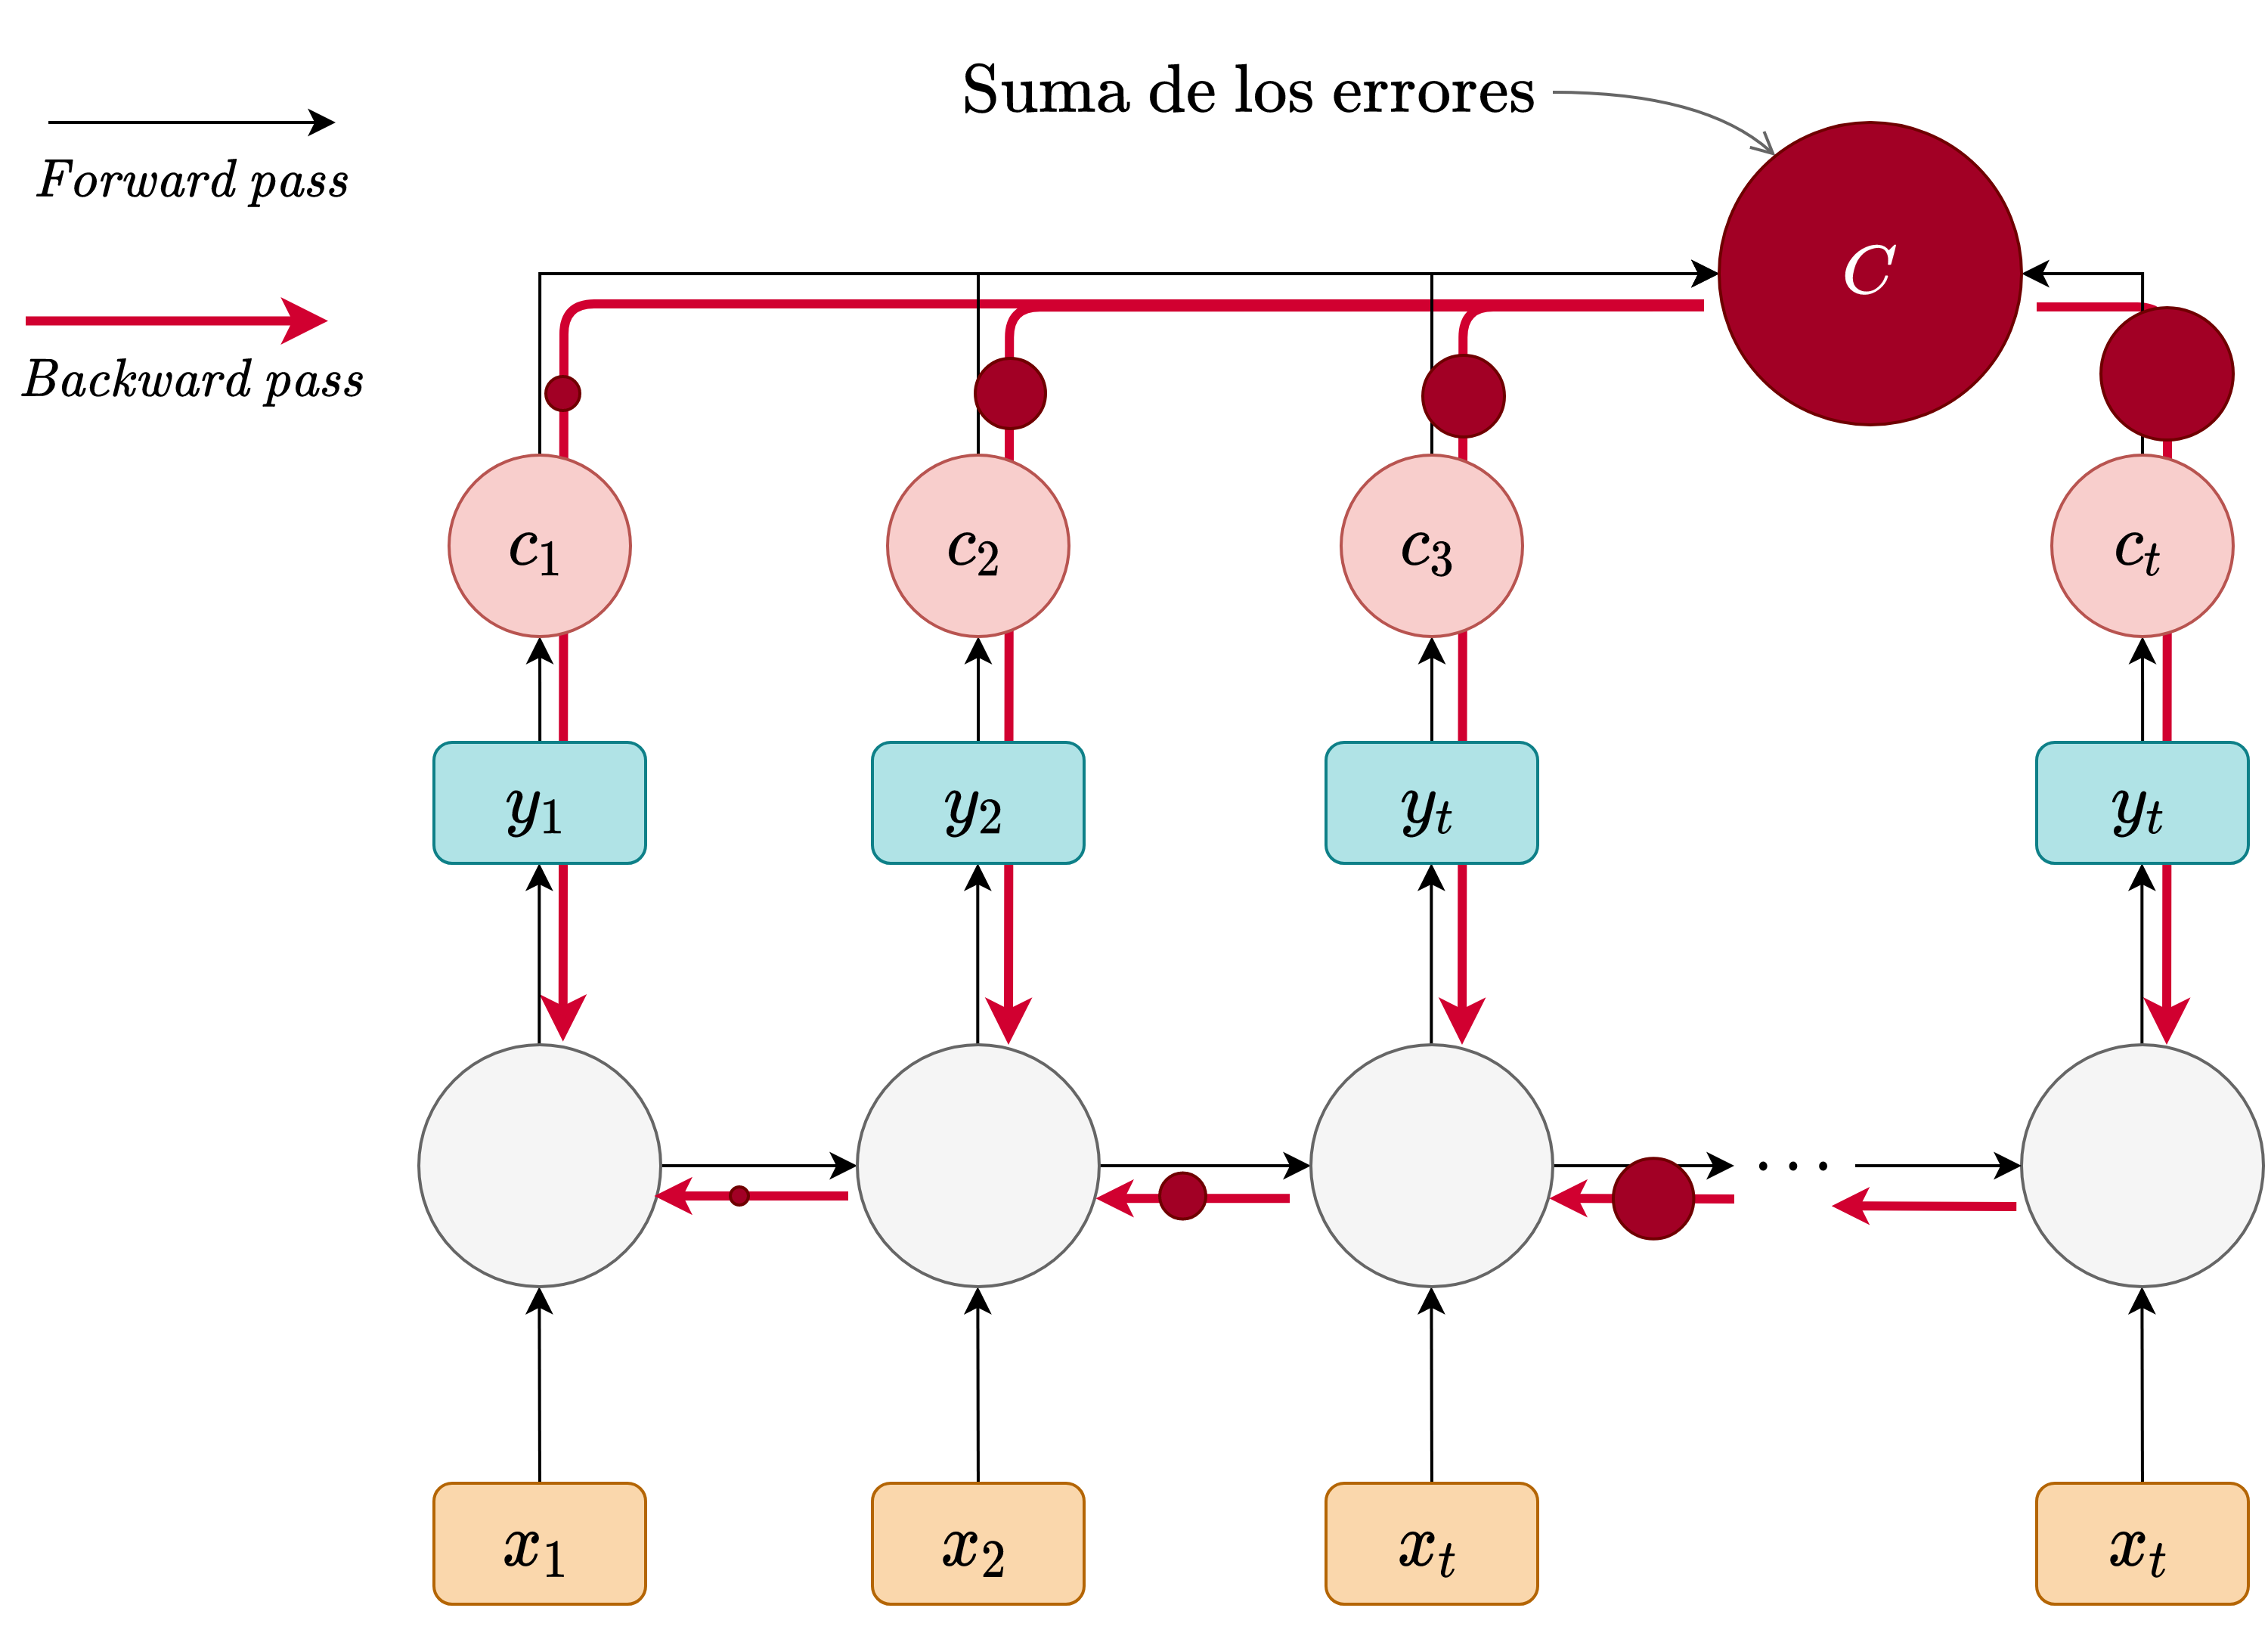
\includegraphics[width=14cm]{images/state-of-art/rnn/rnn-backward.png}
    \caption{\textit{Backpropagation} a través del tiempo en \acrshort{rnn}}
    \label{fig:Backpropagation_through_time}
\end{figure}

Como se puede ver, el error calculado $C$ a partir de todas las $c_i$, fluyen hacia atrás en el tiempo.
Para la primera parte del cálculo del \textit{backpropagation} se pueden usar las mismas ecuaciones \ref{eqn:backpropagation_w} y \ref{eqn:backpropagation_b}. En estas ecuaciones se realiza el cálculo del coste respecto a $w$ y respecto a $b$. El coste debe de ser $C$ y no $c_i$. Para las capas recurrentes, habrá que calcular una nueva derivada: $\frac{\partial c}{\partial W_H}$. Aplicando la \textit{chain-rule} como se ha explicado en la sección \ref{backpropagation}.

\begin{equation}
\begin{split}
     \frac{\partial C}{\partial W_h} &= \frac{\partial C}{\partial z^{L_i}} \cdot \frac{\partial z^{L_i}}{\partial W_h}
\end{split}
\label{eqn:backpropagation_h}
\end{equation}

Y al igual que en el cálculo del gradiente que se ha realizado para $w$ y para $b$ en la ecuación \ref{eqn:gradients}, se tiene que calcular el gradiente de $W_H$ de la misma forma:
\begin{equation}
    \nabla f_{w_h} = \begin{pmatrix} \frac{\partial C}{\partial w_h^{RL_1}}, & \frac{\partial C}{\partial w_h^{RL_2}}, & \cdots , &  \frac{\partial C}{\partial w_h^{RL_n}} \end{pmatrix}
\end{equation}

Un detalle a recalcar es que se está usando $w_h$ y no $W_H$, puesto que esta última hace referencia a la matriz de pesos de la capa recurrente. El gradiente se debe de calcular de forma independiente por cada neurona, al igual que ocurre con $w$ y $W$. Este concepto se explica con más detalle en la Sección \ref{workingwithmatrixes}. Una vez calculado todos $\nabla f_h$ para cada neurona, se puede actualizar la matriz de pesos $w_{H}$:
\begin{equation}
    \begin{split}
    H^* = H - \eta * \nabla f_{w_h}
    \end{split}
\end{equation}

Es importante primero realizar el cálculo del \textit{backpropagation} y posteriormente realizar el cálculo del gradiente.
\newline
